\documentclass[11pt, a4paper, twoside, headsepline]{scrreprt}
\usepackage{scrpage2} 
%\usepackage{perpage} %make footnotes per page
%\MakePerPage{footnote}
\usepackage[utf8]{inputenc}
\usepackage[swedish,english]{babel}
\usepackage[T1]{fontenc}
\usepackage{lmodern}
\usepackage{amsmath}
\usepackage{fixmath}
\usepackage{graphicx}
%\usepackage{xcolor}
%\usepackage{textcomp}
\usepackage[usenames,dvipsnames]{color}
\usepackage[small,font=it]{caption}
\usepackage{amssymb}
\usepackage{units}
\usepackage{upgreek}
\usepackage{icomma}
%\usepackage{pdfpages}
\usepackage{cite}
\usepackage{listings}
\usepackage{units}
%\usepackage[sc]{titlesec}
%\usepackage{fancyhdr}
\usepackage[breakall,fit]{truncate}
\usepackage[intoc,refpage]{nomencl}
\usepackage{lettrine}
\usepackage{geometry}
\usepackage{eso-pic}
\usepackage{titling}
\usepackage{multirow}
\usepackage{chngcntr}
\usepackage{amsthm}
\usepackage{subfig}
\usepackage{lmodern}


\newcommand{\floor}{\mathrm{floor}}

\setkomafont{disposition}{\bfseries}

\renewcommand{\headfont}{\fontsize{12}{12}\selectfont\normalfont\slshape}

    \makeatletter
    \renewcommand{\@makechapterhead}[1]{%
    \vspace*{50 pt}%
    {\setlength{\parindent}{0pt} \raggedright \normalfont
    \bfseries\Huge\thechapter.\ \, #1
    \par\nobreak\vspace{40 pt}}}
    \makeatother






\usepackage{upref}
\newcommand{\footnoteindex}[1]{\setcounter{footnote}{#1}\addtocounter{footnote}{-1}\footnotemark}
\newcommand{\footnoteref}[1]{Footnote #1}



\newcommand{\backgroundpic}[3]{%
\put(#1,#2){
		\parbox[b][\paperheight]{\paperwidth}{%
			\centering
			\includegraphics[width=\paperwidth,height=\paperheight,keepaspectratio]{#3}
			\vfill
}}}

\newcommand{\mail}[1]{\href{mailto:#1}{\nolinkurl{#1}}}

%\pagestyle{fancy}
%\lhead{\truncate{16em}{\fontsize{10}{11}\selectfont\rightmark}}
%\rhead{\truncate{20em}{\fontsize{10}{11}\selectfont\leftmark}}
%\lhead{\rightmark}
%\rhead{\leftmark}
%\setlength{\headheight}{15pt}

%%% Closed square root
\usepackage{letltxmacro}
\makeatletter
\let\oldr@@t\r@@t
\def\r@@t#1#2{%
\setbox0=\hbox{$\oldr@@t#1{#2\,}$}\dimen0=\ht0
\advance\dimen0-0.2\ht0
\setbox2=\hbox{\vrule height\ht0 depth -\dimen0}%
{\box0\lower0.4pt\box2}}
\LetLtxMacro{\oldsqrt}{\sqrt}
\renewcommand*{\sqrt}[2][\ ]{\oldsqrt[#1]{#2}}
\makeatother
%%%

%%%
\newcounter{myfootnote}
\makeatletter
\@addtoreset{equation}{myfootnote}
\makeatother
\newcounter{myequation}
\makeatletter
\@addtoreset{equation}{myequation}
\makeatother
% Resetting the equation counter is done by stepping myequation, so use \stepcounter{myequation} instead of \setcounter{equation}{0}
% Else, hyperref fails
\newcounter{myfigure}
\makeatletter
\@addtoreset{figure}{myfigure}
\makeatother
\newcounter{mytable}
\makeatletter
\@addtoreset{table}{mytable}
\makeatother
%%%


%\renewcommand\headheight{14pt}


\usepackage[bookmarks, unicode=true, pdftitle={EventGenerators}, pdfauthor={Stefan Buller}, colorlinks=true, linkcolor=black, citecolor=black, urlcolor=black]{hyperref} %assumes black text!

\usepackage[all]{hypcap}
\usepackage[intoc,refpage]{nomencl}
\renewcommand{\nomname}{Glossary} % rename nomenclature
\renewcommand{\nomlabel}[1]{\textbf{#1}}
\makenomenclature

\def\figureautorefname{Figure}
\def\chapterautorefname{Section}
\def\sectionautorefname{Section}
\def\subsectionautorefname{Section}
\def\subsubsectionautorefname{Section}
\newcommand{\subfigureautorefname}{\figureautorefname}

\newenvironment{myenumerate}{%
  \edef\backupindent{\the\parindent}%
  \enumerate%
  \setlength{\parindent}{\backupindent}%
}{\endenumerate}


\makeatletter
\newenvironment{tablehere}
  {\def\@captype{table}}
  {}

\newenvironment{figurehere}
  {\def\@captype{figure}}
  {}
\makeatother

\newcommand{\ordo}[1]{{\cal O}\left( #1 \right)}
\newcommand{\im}{\ensuremath{\mathrm{i}}}
\newcommand{\e}{\ensuremath{\mathrm{e}}}
\renewcommand{\d}{\ensuremath{\mathrm{d}}}

\newcommand{\bra}[1]{\langle #1 \mid}
\newcommand{\ket}[1]{\mid #1 \rangle}
\renewcommand{\vec}[1]{\boldsymbol{#1}}

\newcommand{\chem}[2]{\mathrm{#1}_{#2}}
\newcommand{\dfn}[2]{\emph{#1}\footnote{#2}}
\newcommand{\abbrev}[2]{\emph{#1} (#2)}
\newcommand{\E}[1]{\ensuremath{\mathrm{E}[#1]}}

%\newcommand{\prgname}[1]{\textsc{#1}}
%to make smallcaps work in \section, etc. normally a problem because no bold sc
%texorpdfstring to make hyperref give proper side-bar clicky!
 \usepackage{relsize}
  \newcommand{\prgname}[1]{\texorpdfstring{\textsmaller{\MakeUppercase{#1}}}{\textsc{#1}}}


\newcommand{\pM}{\mathrel{\raise -2.2pt \hbox{\tiny(\,}\!
                 \raise 2pt \hbox{+}
                 \settowidth {\dimen03} {+}
                 \hskip-\dimen03
                 \raise -3.4pt \hbox {$-$}
                 \!\raise -2.2pt \hbox{\tiny{\,)}}}}

\newcommand{\codename}{\prgname{Codez}}
\newcommand{\nucl}[3]{
\ensuremath{
\phantom{\ensuremath{^{#1}_{#2}}}
\llap{\ensuremath{^{#1}}}
\llap{\ensuremath{_{\rule{0pt}{.75em}#2}}}
\mbox{#3}
}
}

\title{EventGenerators}
\author{Stefan Buller}
\date{\today}


\begin{document}
% Chalmers title page
\begin{titlepage}
\AddToShipoutPicture{\backgroundpic{-4}{56.7}{titlepageabstract/frontpage}}
\mbox{}
%\vspace{10cm}
\scalebox{0.12}{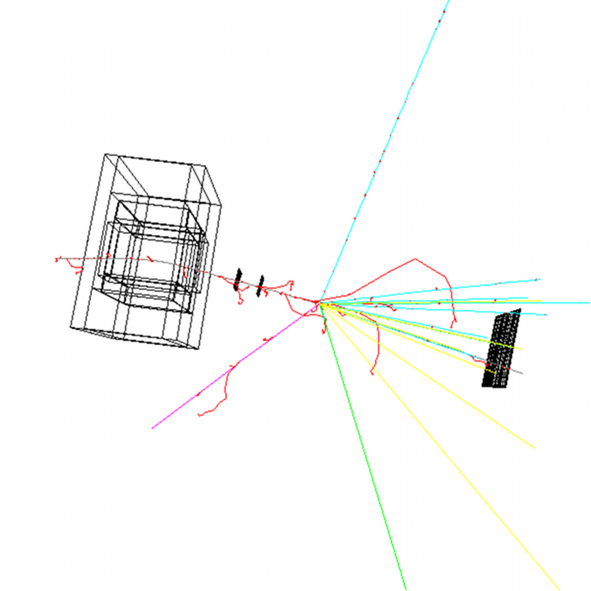
\includegraphics{titlepageabstract/titlefig2.pdf}}
\vfill
%\vspace*{-12cm}
\addtolength{\voffset}{2cm}
\begin{flushleft}
%\vspace*{3cm}
	{\noindent \LARGE{Event Generator for \rtb{}} \\[0.3cm]
	\emph{\Large Master's Thesis in Physics and Astronomy} \\[.8cm]
	
	\Large{STEFAN BULLER}\\[.8cm]
	
	{\Large Department of Fundamental Physics \\
	\textsc{Chalmers University of Technology} \\
	Gothenburg, Sweden 2015 \\
%	Master's Thesis 2011:1\\
	} 
	}
\end{flushleft}
\end{titlepage}
\ClearShipoutPicture
% End Chalmers title page
\pagestyle{empty}
\clearpage
\mbox{}
\clearpage
\thispagestyle{empty}

\thispagestyle{empty}
\begin{titlepage}

\begin{center}
\vspace*{0.5cm}
\huge{\textbf{\thetitle }}
\vspace*{1.5cm}

\Large{\textsc{Master's Thesis}}\\
\vspace*{1cm}
\large{\textsc {by}}\\
\vspace*{0.4cm}
\LARGE{\theauthor}\\
\vspace*{1.2cm}
\Large{\textsc{Supervisors:}}\\
\vspace*{0.4cm}
\LARGE{Andreas Heinz}\\
\vspace*{1.0cm}
\Large{\textsc{Examiners:}}\\
\vspace*{0.4cm}
\LARGE{Thomas Nilsson}
\vfill
\large{Department of Fundamental Physics \\
	Chalmers University of Technology \\
	Gothenburg, Sweden 2015}
\end{center}

\end{titlepage}
\clearpage
\noindent EventGenerators\\
\noindent Stefan Buller (\href{mailto:bstefan@student.chalmers.se}{bstefan@student.chalmers.se})\\\\
\copyright Stefan Buller, 2015.\\\\
FUFX03  - Master's thesis at Fundamental Physics\\
Supervisor: Andreas Heinz\\
Examiner: Thomas Nilsson\\\\
Department of Fundamental Physics\\
Chalmers University of Technology\\
SE-412 96 Göteborg\\
Sweden\\
+46 (31) 772 1000\\\\
Printed by Chalmers Reproservice\\
Göteborg, Sweden 2015
 
\vfill
\noindent{\bf Cover:} The prefered decay modes for various nuclei at an excitation energy of \unit[15]{MeV}, according to the code developed in this project. A red box signifies that the nucleus preferentially decays by emitting a proton, while a blue box means that neutron emission is the most common decay mode. Cyan boxes corresponds to nuclei who deexcite primarily by emitting an alpha particle.
\clearpage
%\begin{minipage}[t][0.50\textheight]{\textwidth}
\subsection*{\centering Abstract}
{\fontsize{10}{11}\selectfont 
This thesis describes various models implemented in a code to simulate nuclear reactions that go through a compound nucleus state, an intermediate excited state long lived enough that the nucleus has time to reach equilibrium between each subsequent decay. This implies that the decay is effectively characterized by macroscopically conserved quantities such as the excitation energy $E^*$ and its spin $J$, in addition to the proton and neutron number, $Z$ and $N$, respectively.

Specifically, the reactions under consideration are quasi-elastic scattering reactions, in which the collision is modeled as taking place between essentially free nucleons or clusters in the target and projectile. A Feynman diagram formalism is used to describe this first, fast knock-out reaction.
The unaffected nucleons in the projectile will then form an excited compound nucleus, and the final reaction products are determined by decaying this compound system. 

The codes to simulate the initial fast reaction and subsequent decay are separate programs. Results are presented regarding the prefered decay modes of nuclei with a given excitation energy, utilizing the decay part of the code. The results obtained for an excitation energy of $\unit[20]{MeV}$ were compared with the output of another program, \prgname{Talys}, for nuclei with $Z\in [10,90]$ and $N \in [10,130]$. 

Finally, the quasi-elastic scattering code and the compound nucleus deexcitation code were coupled in order to allow the code to be used as an event generator. The output of the event generator was used in simulations to benchmark the performance of the addback algorithm used to determine gamma energies and multiplicites from actual experimental data. The tentative results indicate that the addback algorithm is unable to identify the number of $\gamma$-rays emitted in the reaction, although further investigations are needed to arrive at a conclusive result.
}
%\end{abstract}
%\end{minipage}
%\vspace{-3cm}

\selectlanguage{english}
\thispagestyle{empty}

\chapter*{Acknowledgements}
%Lorem ipsum dolor sit amet, consectetur adipisicing elit, sed do eiusmod tempor incididunt ut labore et dolore magna aliqua. Ut enim ad minim veniam, quis nostrud exercitation ullamco laboris nisi ut aliquip ex ea commodo consequat. Duis aute irure dolor in reprehenderit in voluptate velit esse cillum dolore eu fugiat nulla pariatur. Excepteur sint occaecat cupidatat non proident, sunt in culpa qui officia deserunt mollit anim id est laborum. 

\thispagestyle{empty}
This project would not have started or finished without Andreas Heinz, who both suggested the topic and provided support and supervision throughout this project.

The \prgname{Talys} simulations, which were used to partially compare the output of the code, would obviously not have been possible without the \prgname{Talys} team. In particular, I am indepted to Arjan Koning for being helpful over mail, providing me with the latest version of \prgname{Talys}, and for adding a \prgname{Talys} keyword that enabled me to do the comparison between the emission spectra of my program and \prgname{Talys}.

Also good at alleviating technology related pain is Håkan Johansson, who (mostly) has kept the computers at the subatomic physics group happy.

On the few occasions when the computers weren't happy, I could usually blame Simon Lindberg, who -- in addition to tormenting the intranet -- inspired me to have a look at gamma-multiplicites and explained the addback routine used to analyze the energy deposits in the Crystal Ball detector.

Last but not least, I would like to thank the entire subatomic physics group for bearing with me and making me feel welcome -- and the University for all the cake.
\\[1cm]

\hfill Stefan Buller, Gothenburg, June 2015
\clearpage
\pagenumbering{roman}



\selectlanguage{english}


%\setcounter{page}{1}
\tableofcontents
\clearpage

\pagestyle{scrheadings}
\automark[section]{chapter}
\ofoot[\pagemark]{\pagemark}
\cfoot[]{}

\setlength{\oddsidemargin}{8pt}
\setlength{\evensidemargin}{23pt}

%notation page
%\input{notations/notations.tex}

\newpage
\pagenumbering{arabic}
\setcounter{page}{1}
\chapter{Introduction}
\label{sec:intro}
%\nomenclature{intro}{an introduction}
As a part of the construction of international FAIR (Facility for Antiproton and Ion Research), the LAND experimental setup is succeeded by the \rtb{} (Reactions with Relativistic Radioactive Beams) setup, which includes a score of new detectors. During all stages of this process---from designing and calibrating the new individual detectors and the entire setup, to analyzing the data and extracting the underlying physics---simulations are or will be used. 

The \rtb{} experiment aims to study nuclear physics, in particular the properties of exotic nuclei far from the valley of stability \cite{r3b:online}. The experiments will be performed with radioactive beams, and the aim is to be able to determine the complete kinematics of the reaction. We will here describe a generic experiment of this kind.

The radioactive beam impinges on a target surrounded by detectors. In the case of a reaction at the target---a so called \emph{event}---the reaction products are, ideally, identified by recording where they hit the detector, when they hit the detectors (which allows detector output to be attributed to individual events, which yields the initial and final momentum); how much energy they deposit in the detectors (yielding the charge); and their deflection in a magnetic field, which gives their charge-to-mass ratio, and thus their mass. 

This is of course a simplification: the reaction products may decay in-flight, they may be deflected by interacting with the air, or a detector. This is why simulations are used, specifically Monte-Carlo simulations, since the underlying physics is non-deterministic. 

While simulations are used to determine how a given reaction product propagates throughout the experimental setup, they are not necesarilly needed for the actual reactions at the target, since the purpose of the experiment is to investigate those. 
In many cases, this is not a problem: it is enough to simulate particles with specified initial momenta matching the kinematic constraints of the reaction and see how they propagate through the experimental setup---a setup which should be able to identify them even if they are not the result of an actual reaction.
However, since the setup in practice only should identify actual reactions products, it would be more ideal if the simulations incorporated some of the theory around the reactions to be studied.

\section{Event Generator for \rtb{}}
As mentioned in the previous section, an experimental event is a reaction between the target and the beam.
An \emph{event generator}, on the other hand, is in this context a piece of code that mimics certain reactions for the simulation codes. The output of such an event generator would be final state momenta and energies of the reacting particles, which can then be propagated through the simulated experimental setup. %In principle, an event generator could also give initial positions for the particles to be propaged, but since the reactions takes place on a negliable length scale, compared to the experimental setup, this is in practice not needed.

In principle, one can think of an event generator that exactly simulates the reactions at the target and returns a final state with a probability mimic the experiment. However, there are good reasons to not implement this event generator, not all of them related to how unfeasible that project would be---considering our present knowledge of nuclear physics. In the remainder of this section, I will try to arrive at some design principles for a feasible event generator.

!!!I AM USING 'I' HERE SINCE I BELEIVE THIS TO BE LESS OF AN OBJECTIVE CONCLUSSION. I'M NOT 100\% SURE ABOUT THIS, THOUGH!!!

\subsection{Design of an event generator}
Before I argue for why a completely realistic event generator may be undesirable, let me first mention a few reasons for why it is unfeasible---it will turn out that one of these reasons is closely related to why a 'sloppy' event generator is useful.

Firstly, the nucleon-nucleon interaction is not well understood from first principle: there is no one model for the atomic nucleus. Even with our best understand of the interaction between individual nuclei, calculations with even moderately sized systems require supercomputer resources. !!!CITE SOMETHING ABOUT LIMITS OF THIS APPROACH WITH CURRENT RESOURCES. DEFINE ``MODERATELY SIZED SYSTEM''!!!
It is thus clear that another approach is needed for the implementation of an event generator, especially if we add the constraint that it should be possible to run on an ordinary computer.

There exist a number of more-or-less phenomenological models to describe nuclear reactions from a simpler perspective, i.e. one that does not require a super computer. I will describe a few such models in more detail in \autoref{sec:theory:nuc-col}. 

Numerous codes have been written to simulate nuclear reactions. A recent article by Kara et. al.\cite{kara:2015:art} has compared simulation output from three widely used codes, \prgname{Empire}\footnote{\url{http://www.nndc.bnl.gov/empire/}, available as of 2015-04-17.}, \prgname{Talys}\footnote{\url{http://www.talys.eu/home/}, available as of 2015-04-17.}, and \prgname{Alice/ash}\footnote{\url{http://bibliothek.fzk.de/zb/berichte/FZKA7183.pdf}, avaliable as of 2015-04-17 is the best reference I can find right now...} and experimental data: 


%\begin{itemize}
%\item Computational time
%\item Model dependence
%\item Rare events
%\end{itemize}



\chapter{Theoretical Background}
\label{sec:theory}

\chapter{The Code}
\label{sec:code}
The \codename{} code, based on CODEX\cite{gollerthan:1988:thesis}, contains models for the various quantities needed in statistical models. It is written to be extendable and to a large extent modular, so that the various models can easily be replaced. Details on the specific models may be found in \autoref{sec:theory:nuc-col}.
To achieve this modularity, the code is written in C++ and makes use of \emph{object-oriented} programming concepts. 

The program is roughly structered as follows:
 Decay processes are specified by model objects, which contain models for calculating transition probabilities to possible final states. ``Probabilities'' here refers to $d^2 P_\nu/dtdE$, roughly the probability to decay to a final state in energy interval $dE$ during the time $dt$ by the process $\nu$. The probabilities need not be normalized.
The model objects implement a function that for a given energy discritization tabulates a specification of the decay (The excitation energy of the final state, the spin of the final state, the particle $\nu$ which was emitted in the decay, its orbital angular momentum) along with a corresponding cummulative probability. A complete table of cummulative transition probabilities and final states is generated by looping over all model objects.

 A de-excitation step may then be performed by drawing a random number between $0$ and the final cummulative probability, and looking up the corresponding decay in the table. Several one-step decays from the same state may thus be performed with little extra computational costs.

The tabulation of decay probabilities, the deexcitation and the models all compile to different object-files, which are linked to produce exectable files with various purposes -- such as deexciting a nucleus until its excitation energy reaches a certain value, finding the most common decay channel for several different nuclei with given excitation energies, export level densities, etc. 
This removes the need to excessively control the program flow in the individual main-files, which makes the code easier to read, since it mostly describes the physics -- although it may lead to some code duplication.

The next section describes the individual executable programs, and demonstrates how they may be used together to solve more complicated tasks.

\section{Programs}
The \codename{} code contains three types of subprograms: programs to generate list of nuclei, programs that run on a list of nuclei, and programs that process the output of the latter programs.
The different kinds of programs may be used in a pipe, like
\begin{lstlisting}[language=bash]
list | run | process
\end{lstlisting}

\subsection{List generating programs}
The first kind of program simply generate lists of nuclei to perform calculations for. The output of these programs are on the form illustrated by this example output:
\begin{lstlisting}
#comment
*Event 1
Z11 N11 E11 J11 px11 py11 pz11
Z12 N12 E12 J12 px12 py12 pz12
*Event 2
Z21 N21 E21 J21 px21 py21 pz21
\end{lstlisting}
where $Z,N,E,J,p$ specify the proton number, neutron number, excitation energy, spin and 3-momentum of the nucleus. If no event numbers are present, each line is assumed to be a separate event. Simpler lists could easily be written by hand, but the list-type programs make it possible to easily run a specific calculation (as specified by a ``run-type'' program) for a range of nuclei, or nuclei generated by a specific process.

\subsubsection{\prgname{Nuclist}}
The \prgname{Nuclist} program simply generates a list of nuclei for a given $N$, $Z$ or $A$ range; with a given excitation energy, spin and initial momentum. This program can be used to determine spectra from excited nuclei of certain isotopes, isobars and isotones.

Each nuclei is placed in a separate event.

\subsubsection{\prgname{Quasi}}
This program simulates a quasi-elastic scattering event, producing an excited prefragment as well as the participant knocked-out cluster and target fragment.
The beam energy, the number of events, the participant nuclei must be specified, and the excitation energy and spin of the spectator prefragment may be specified.

The target and cluster fragments are assumed to be unexcited, which should be a good assumption for p2p reactions.

Each scattering event is placed in a separate event.

\subsection{Programs to run on nuclei-lists}
These programs can be run on a list produced by the above programs in order to perform various calculations. 

\subsubsection{\prgname{Spectra}}
This program, primarily intended to be run on the output of \prgname{Nuclist}, prints the probabilities of various decay modes from the initial states specified by the nuclie-list. The \texttt{--details} flag controls to which level of detail the spectra are printed. This is essentially a program to illustate the decay widths as calculated by the program, and hence it ignores event numbers.

\subsubsection{\prgname{Deexcite}}
The bulk work of an event generator is performed in this program. Each nuclei in each event in the input file is deexcited until it is below a specified threshold energy, or for a given number of deexcitation steps, and the resulting nuclei are printed to a new list, with the event number inherited from their mother nuclei. Combined with the output of \prgname{Quasi} and the post-processing program \prgname{List2gun}, this program is able to act as an event generator for \prgname{Geant4} through the wrapper \prgname{ggland}.

\subsubsection{\prgname{Rho}}
This program produces a \emph{tab-separated value} (tsv) file of the level density for each nuclei in the input list. By default, only the $Z, N$ and $J$ of the nuclei is used, and the level density is plotted for a range of excitation energies, rather than the actual energy of the nuclei in the input files, which are ignored in this mode.

\subsubsection{\prgname{Pot}}
Like \prgname{Rho}, this program produces a \emph{tab-separated value} (tsv) file for each nuclei in the input list, this time of the potential a particle has to tunnel through to be emitted by the nuclei in the list. The potential for a given particle-decay can be exported for a range of $l$ values.

%\subsection{Transition Probabilities}
%The transition probability $d^2 P_\nu/dtdE$ from an initial state $i$ to a final state $f$ by the process $\nu$ is roughly given by
%\begin{equation}
%R \equiv \frac{d^2 P_\nu}{dtdE} = \sum_j \frac{\rho_{f}}{\rho_i} T_{\nu,j}(E_i,E_f).
%\end{equation}
%Here, $\rho$ is the nuclear level density for the initial and final states, $T_{\nu,j}(E_i,E_f)$ the transmission coefficient, with $j$ being a collective index describing the diffrent ways a process may carry the nucleus from $i$ to $f$.
%\label{sec:theory}
%\input{physics/physics.tex}



\printnomenclature
\bibliography{bibli}{}
\bibliographystyle{joelspropack}

\newpage
\appendix
\stepcounter{myequation}
\counterwithin{equation}{chapter}
\chapter{Appendix 1}
\label{app:brho}

\chapter{Code}
\label{app:code}

\lstset{language=C++ ,basicstyle=\footnotesize, breaklines=true, %backgroundcolor=\color[rgb]{0.8,0.8,0.8},
xleftmargin=11pt, xrightmargin=11pt
}
\begin{lstlisting}
struct spec_POS_t
{
  SPEC_FLOAT(_dx,             2.5,"cm","full width x of active volume");
  SPEC_FLOAT(_dy,             2.5,"cm","full width y of active volume");
  SPEC_FLOAT(_dz,          0.03,"cm","full width z of active volume");
  SPEC_FLOAT(_lgheight,     2,"cm","lightguide height over active volume");
  SPEC_FLOAT(_lgheadd,     0.70,"cm","size of square-shaped lightguide-heads");
  SPEC_MEDIA(_type,   "plastic",""  ,"POS active volume material.");
  SPEC_MEDIA(_lgtype, "plastic",""  ,"Lightguide material");
};


#include "auto_gen/spec_info_pos.hh"

#define UNUSED_PARAM(x)
\end{lstlisting}
This function is called when \prgname{ggland} creates the detector.
\begin{lstlisting}
gg_geom_obj *make_POS(void *vspec,uint32_t UNUSED_PARAM(mask_set)
		     ,const transform_matrix *loc_rot
		     ,det_name_no_info *name_no)
{
\end{lstlisting}


\clearpage
%initialize SWEDEN!
\counterwithout{equation}{chapter}
\def\figureautorefname{figur}
\def\appendixautorefname{avsnitt}
\def\chapterautorefname{avsnitt}
\def\sectionautorefname{avsnitt}
\def\subsectionautorefname{avsnitt}
\def\subsubsectionautorefname{avsnitt}
\selectlanguage{swedish}
\def\equationautorefname{ekvation}
\stepcounter{myequation}
\stepcounter{myfigure}
\stepcounter{mytable}
\stepcounter{myfootnote}
\renewcommand{\abbrev}[2]{#1\footnote{#2}}
\chapter{Svenska här}
\end{document}

